\documentclass{article}
\usepackage{tikz}
\usepackage{amsmath}
\usepackage{calc}
\usepackage{xcolor}
\usepackage{graphicx}
\usepackage{listings}

\begin{document}
\title{Integral Area}
\author{Made By Kenzy}
\date{\today}

\maketitle
\section{Introduction \& Questions Of The Integral Area}
\nopagecolor 
\subsection{What is integral area?}
\textbf{Integral Area:}
The integral area refers to the area under a curve obtained by evaluating a definite integral. It represents the total enclosed area between the curve, the x-axis, and the interval of integration. The integral area can be positive or negative depending on the function's behavior within the interval. Integration techniques are used to calculate the integral area, which quantifies quantities such as displacement, value, or change associated with the function or process being modeled.
\begin{equation}
    \int_a^b f(x) \, dx
\end{equation}
\subsection{Who invented integral area?}
The concept of integral area was developed by Sir Isaac Newton and Gottfried Wilhelm Leibniz in the late 17th century.
\begin{figure}[ht]
    \centering
    
\includegraphics[width=0.6\textwidth]{Isaac Newton and Gottfried.jpg}
    \caption{Image depicting the integral area.}
    \label{fig:integral_area}
    \vspace{10pt}
    \small Isaac Newton and Gottfried
\end{figure}
\section{What is it used for?}
The integral area has various applications, including calculating areas, quantifying physical quantities, solving differential equations, probability and statistics, optimization problems, and applications in physics and engineering. Additionally, it plays a fundamental role in the development of calculus and mathematical analysis.

\subsection{Example: Calculating Work}
One practical application of the integral area is in calculating work done by a force. In physics, work is defined as the product of the force applied to an object and the distance over which the force acts. Mathematically, work can be calculated as the integral of the force function over a given interval.

For instance, consider a force $F(x)$ applied to an object moving along the x-axis from $x = a$ to $x = b$. The work done by the force can be calculated using the integral area as follows:
\begin{figure}[ht]
    \centering
    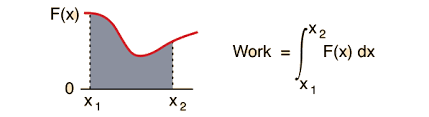
\includegraphics[width=0.6\textwidth]{Work.png}
    \caption{Calculating Work}
    \label{fig:integral_area}
    \vspace{10pt}
\end{figure}

By evaluating this integral, we can determine the total work done by the force on the object over the interval $[a, b]$.

This is just one example of how the integral area is used to calculate physical quantities in real-world applications.

\subsection{Application: Finding Average Value}
Another important application of the integral area is in finding the average value of a function over an interval. The average value represents the constant value that, if maintained over the interval, would result in the same integral area as the original function.

Mathematically, the average value of a function $f(x)$ over the interval $[a, b]$ can be calculated using the integral area as follows:

\begin{equation}
    \text{Average Value} = \frac{1}{b-a} \int_{a}^{b} f(x) \, dx
\end{equation}

By evaluating this integral and dividing it by the length of the interval, we obtain the average value of the function over that interval. \\\
This concept is particularly useful in areas such as signal processing and statistics, where it allows us to represent the overall behavior of a function over a specific range.

This is just one example of how the integral area is used to calculate average values of functions in various fields.

\section{Graphical Representation}

The integral area, a fundamental concept in calculus, refers to the total enclosed area under a curve within a specific interval. This graphical representation vividly illustrates the integral area and its significance. 

\begin{center}
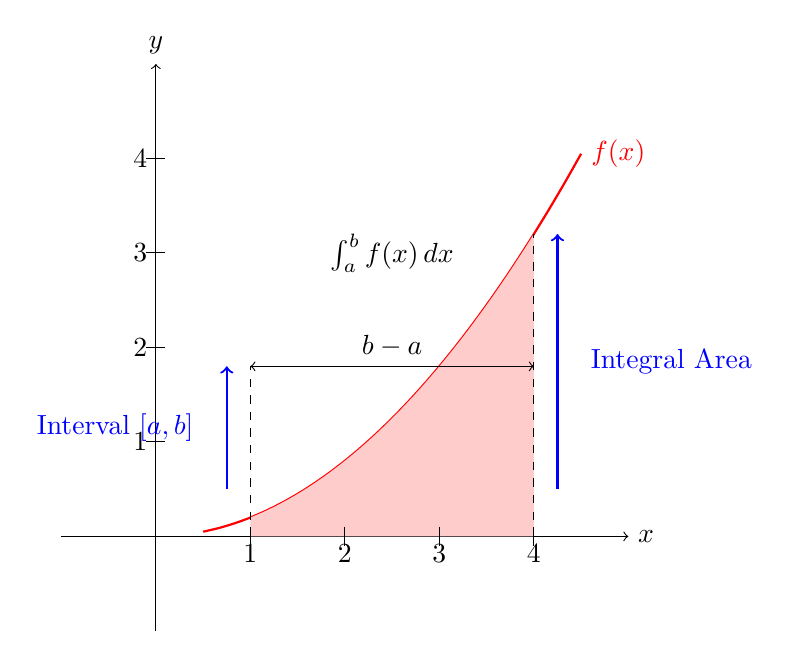
\begin{tikzpicture}[scale=1.2]
  % Axis
  \draw[->] (-1,0) -- (5,0) node[right] {$x$};
  \draw[->] (0,-1) -- (0,5) node[above] {$y$};
  
  % Function
  \draw[thick, domain=0.5:4.5, smooth, variable=\x, red] plot ({\x}, {0.2*\x*\x}) node[right] {$f(x)$};
  
  % Integral area
  \fill[red!20] (1,0) -- plot[domain=1:4, smooth, variable=\x] ({\x}, {0.2*\x*\x}) -- (4,0) -- cycle;
  
  % Axis labels
  \foreach \x in {1,2,3,4}
    \draw (\x,-0.1) -- (\x,0.1) node[below=3pt] {\x};
  \foreach \y in {1,2,3,4}
    \draw (-0.1,\y) -- (0.1,\y) node[left=3pt] {\y};
  
  % Integral notation
  \draw (2.5,3) node {$\int_a^b f(x) \, dx$};
  \draw[dashed] (1,0) -- (1,1.8) (4,0) -- (4,3.2);
  \draw[<->] (1,1.8) -- (4,1.8) node[midway, above] {$b-a$};
  
  % Definitions
  \draw[->, thick, blue] (0.75,0.5) -- (0.75,1.8);
  \draw (0.5,1.15) node[left, blue] {Interval $[a, b]$};
  \draw[->, thick, blue] (4.25,0.5) -- (4.25,3.2);
  \draw (4.5,1.85) node[right, blue] {Integral Area};
\end{tikzpicture}
\end{center}
\section{Conclusion}

In conclusion, the integral area is a fundamental concept in calculus. It represents the total enclosed area under a curve within a specific interval and has various applications in physics, engineering, statistics, and other fields.

By evaluating definite integrals, we can calculate physical quantities, solve differential equations, perform optimizations, and make predictions. The graphical representation of the integral area helps visualize the relationship between the function, the interval of integration, and the enclosed area.

Overall, the integral area is a powerful tool that plays a crucial role in understanding and solving a wide range of problems. It serves as a cornerstone of quantitative reasoning and problem-solving, making it essential for anyone delving into the depths of mathematics and its applications.

\section{Code Implementation}
The following C++ program calculates the integral of a function over a given interval using numerical methods.

\begin{lstlisting}[language=C++, backgroundcolor=\color{blue!5}, basicstyle=\footnotesize]
double function(double x) {
    return x * x;
}

double calculateIntegral(double a, double b, int numIntervals) {
    double h = (b - a) / numIntervals;
    double integral = 0.0;

    for (int i = 0; i < numIntervals; i++) {
        double x1 = a + i * h;
        double x2 = x1 + h;
        double y1 = function(x1);
        double y2 = function(x2);

        integral += (y1 + y2) / 2.0 * h;
    }

    return integral;
}
\end{lstlisting}


In this code, the function \textcolor{blue}{\texttt{function}} calculates the value of the function $f(x)$. Modify the function definition according to your specific function. \\

The \textcolor{blue}{\texttt{calculateIntegral}} function uses the trapezoidal rule to estimate the integral. It takes three parameters: \textcolor{blue}{\texttt{a}} and \textcolor{blue}{\texttt{b}} as the lower and upper limits of the interval, and \textcolor{blue}{\texttt{numIntervals}} as the number of intervals. \\

Inside the function, the width of each interval (\textcolor{blue}{\texttt{h}}) is calculated as the difference between \textcolor{blue}{\texttt{b}} and \textcolor{blue}{\texttt{a}} divided by \textcolor{blue}{\texttt{numIntervals}}. The \textcolor{blue}{\texttt{integral}} variable is initialized to zero. \\

The for loop iterates over each interval. In each iteration, the left and right endpoints of the interval (\textcolor{blue}{\texttt{x1}} and \textcolor{blue}{\texttt{x2}}) are calculated, and the corresponding function values (\textcolor{blue}{\texttt{y1}} and \textcolor{blue}{\texttt{y2}}) are obtained. The area of the trapezoid formed by the interval is added to the \textcolor{blue}{\texttt{integral}} variable. \\

Finally, the function returns the calculated integral. \\
 
Modify this code according to your specific function and requirements for numerical integration. 

\end{document}
